\documentclass[twoside,11pt,a4paper]{article}
\usepackage[margin=2.5cm, bindingoffset=1.25cm]{geometry}
\usepackage{lmodern}
\usepackage[T1]{fontenc}
\usepackage[utf8]{inputenc}
\usepackage[magyar]{babel}
\usepackage[table]{xcolor}
\usepackage{pdfpages}
\usepackage[
	backend=biber,
	style=ieee,
	texencoding=utf8,
	bibencoding=utf8,
	sortlocale=hu
]{biblatex}
	\usepackage{csquotes}
\usepackage{setspace}
\usepackage{enumitem}
\usepackage{titlesec}
\usepackage[babel=true,tracking=true,kerning=true]{microtype}
\usepackage{amsmath}
\usepackage{amsthm}
\usepackage{amssymb}
\usepackage{enumitem}
\usepackage{tikz}
\usepackage[hidelinks, unicode]{hyperref}

\usetikzlibrary{positioning,shapes,arrows,backgrounds,fit}


\DeclareQuoteStyle{magyar}%
  {\quotedblbase}
  [\guillemotleft]
  {\textquotedblright}[0.05em]
  {\guillemotright}
  [\guillemotleft]
  {\guillemotleft}

\addbibresource{biblio.bib}

\sloppy
\frenchspacing
\onehalfspacing
\setlist{noitemsep}

\theoremstyle{plain}
\newtheorem*{defn}{Definíció} 

\newcommand{\cls}[1]{\texttt{#1}}

\newcommand{\plang}[1]{{\color{blue}\texttt{#1}}}
   
\begin{document}
\pagestyle{empty}
\pagenumbering{roman}
\begin{titlepage}
\newlength\drop
\setlength\drop{0.08\textheight}

\centering
\vspace*{2\drop}

{\huge A PLanG programozási nyelv kiterjesztése}\\[\baselineskip]
{Önálló laboratóriumi beszámoló}\\[\baselineskip]

\vspace*{0.5\drop}
\large 2015.

\vfill
\begin{flushright} \large
\emph{Készítette:}\\
Scipiades Ármin\\[\baselineskip]
\emph{Konzulens:} \\
Dr.~Feldhoffer Gergely
\end{flushright}
\vspace*{\drop}

\end{titlepage}
\newpage

\vspace*{\fill}
\begin{center}
A beszámoló elektronikus formában a\\
\url{http://users.itk.ppke.hu/~sciar/onlab.pdf}\\
címen érhető el.
\end{center}

\cleardoublepage
%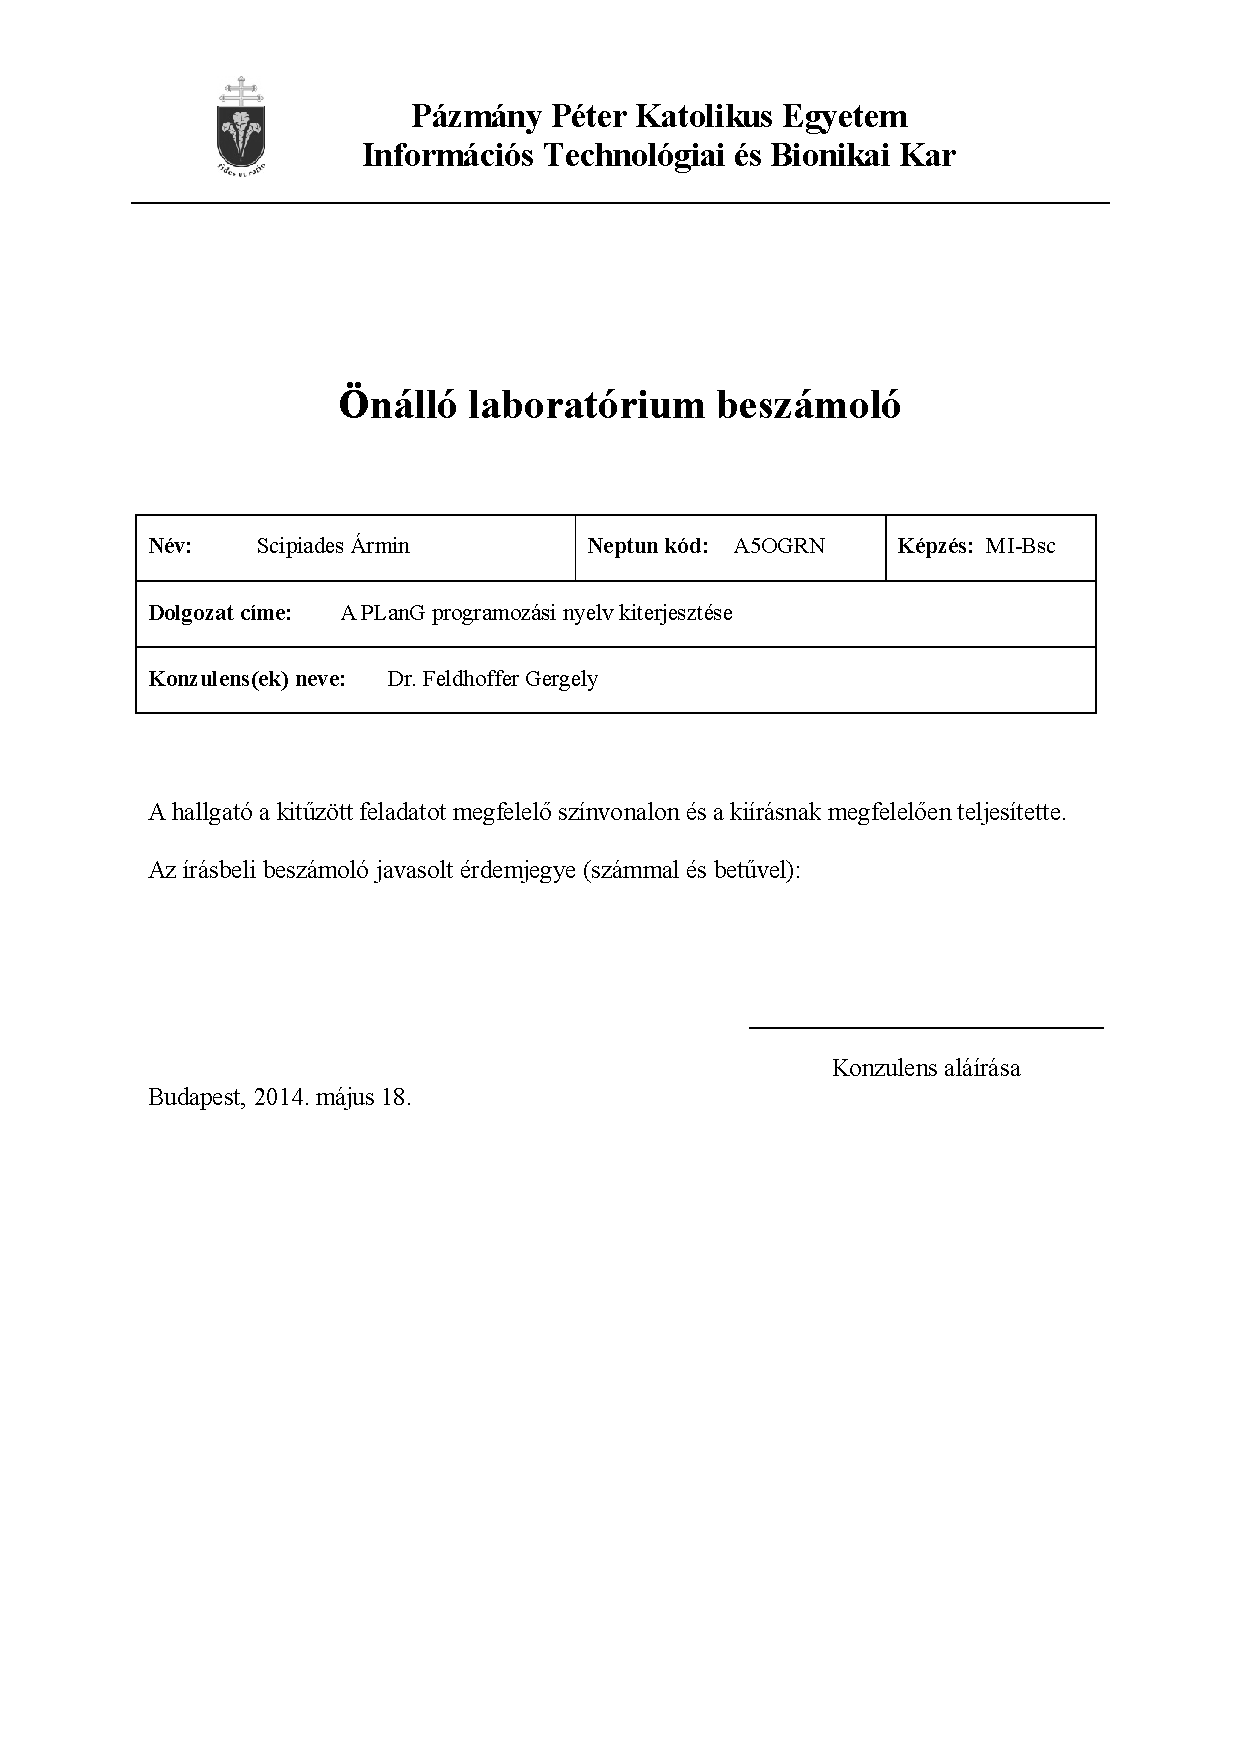
\includepdf{parts/elolap.pdf}
%\cleardoublepage
\tableofcontents

\newpage
\setcounter{page}{1}
\pagestyle{plain}
\pagenumbering{arabic}
\section{Programozási nyelvek}
\label{sec:proglang}
A programozási nyelv algoritmusok leírására szolgáló formális jelölésrendszer, amelyet emberek és számítógépek is értelmezni tudnak.
A programozási nyelv szolgálhat ember és gép közötti kommunikáció eszközeként, lehetővé téve a programozónak, hogy a feladatot megoldó algoritmust a számítógép számára érthető módon megfogalmazza.
De a programozási nyelv kommunikációs eszköz lehet ember és ember között is, hiszen a megírt programot a programozón kívül mások is olvasni fogják majd, akár mert javítaniuk kell a programon, akár mert tovább akarják fejleszteni, akár mert tanulni akarnak belőle.


\subsection{Történeti áttekintés}
Az embernek és a gépnek a közös nyelvvel szemben támasztott igényei jelentősen eltérnek.
Kezdetben, a számítógépek megjelenésekor egyértelműen a gépek igényei voltak előtérben: a programozónak ténylegesen a gép nyelvén kellett beszélnie, \textbf{gépi kód}ban kellett közölnie a gondolatait, vagyis ténylegesen bináris számok sorozataként kellett megírnia a programját, ahol minden szám egy-egy gépi utasítást, illetve az utasítás operandusaiként szolgáló memóriacímeket jelölte.
Ez nagyon távol áll az emberi gondolkodástól, a természetes nyelven kifejezett algoritmustól: a program lefordítása a gép nyelvére a programozó igen nehéz és munkaigényes feladata volt, a program olvasása pedig hasonlóan nehéz.

Az ember-orientált nyelvek kialakulásának első lépése a csak embereknek szánt programleíró jelölésrendszerek megjelenése volt: Konrad Zuse \textit{Plankalkül}je, Neumann János és Herman Goldstine programleíró folyamatábrái, Currie lambda-kalkulusa voltak az első olyan rendszerek, amelyek lehetővé tették algoritmusok formális leírását.
Érdemes megjegyezni, hogy bár a matematika nagyon fejlett eszköztárat épített ki statikus struktúrák leírására, az algoritmusokat egészen addig természetes nyelven adták meg\cite{KnuthTrabbPardo}.

A negyvenes évek végén jelentek meg az első \textbf{assembly-szintű nyelvek}, ahol bináris számok helyett a programozó már rövid nevekkel, mnemonikokkal hivatkozhatott egy gépi utasításra, és konkrét memóriacímek helyett már azonosítókkal hivatkozhatott változókra.
Az így leírt programot táblázatok segítségével könnyű átírni gépi kódra, és ez a fordítási folyamat könnyen automatizálható is: így jelentek meg az assemblerek, az első fordítóprogramok.
Ez volt at első lépés az ember-orientált nyelvek kifejlődése felé: a programozóknak nem kellett többé numerikus utasításkódokat észben tartaniuk vagy memóriacímeket számolniuk, sőt, a fordítóprogram már képes volt bizonyos hibákat felderíteni a kapott programban. És bár az assembly-szintű nyelvekben eleinte a gépi utasítások és az assembly mnemonikok között egy-egy kapcsolat volt, de hamarosan megjelentek az első ,,makrók'', azaz makróutasítások (vagyis szó szeint ,,óriásutasítások'') is,  amelyek több gépi utasításból álló sorozatokat helyettesítettek.
Megjelentek az első szubrutinkönyvtárak is, amelyek lehetővé tették a programozó számára a magasabb absztrakciós szinten való gondolkodást.

Az ilyen korai \textit{autocoding} technikák fejlődésével alakultak ki a \textbf{magasszintű nyelvek}, melyeket architektúrafüggetlenség, a magas absztrakciós szint biztosítása, az assemblyhez képest rövidebb, áttekinthetőbb szerkezetű programok írásának lehetősége jellemez, és az, hogy a nyelv közelebb áll az emberi nyelvhez.
%Az első sikeres magasszintű nyelv a FORTRAN volt, tervezési céljai közül a tömörség és a gyors elsajátíthatóság voltak a lefontosabbak.
Fejlődésükben katalizátorként hatott Noam Chomsky generatív nyelvelmélete, melynek alapján viszonylag komplex nyelvtani struktúrákat hatékonyan felismerő és gépi nyelvre fordító algoritmusokat lehetett kidolgozni.

A magasszintű nyelvek kifejlesztésének motivációja a programozói termelékenység növelése volt\cite{Backus78}, a programozók körében mégis sokáig érezhető volt egyfajta ellenérzés a magasszintű nyelvekkel szemben, mondván, hogy a magasszintű nyelvek emberorientáltsága a \textit{hatékonyság} és a \textit{kreativitás} rovására megy\cite[12.~fejezet]{MythManMonth}.
A számítógépek teljesítményének fejlődésével és az egyre szofisztikáltabb fordítóprogramok megjelenésével ezek a kritikák háttérbe szorultak ugyan, de ezzel párhuzamosan egyre magasabb szintű, egyre emberorientáltabb programozási nyelvek jelentek meg, melyekkel szemben a korábbi magasszintű nyelvek kedvelői fogalmaztak meg hasonló kritikákat.
A \textit{magasszintű nyelv} kifejezés így egyre magasabb szintű nyelvekre utal: az első magasszintű nyelveket egy mai programozó már jórészt alacsonyszintűnek tekinti.
A ma programozója számára ,,túl magas'' szintű programozási nyelvek például a programkódot automatikusan generáló szoftvertervezési eszközök; ezekkel szemben a mai programozók hasonlóan a hatékonyságot és a kreativitást féltik, mint a hatvanas évek programozói a magasszintű nyelvektől\cite{Veto}.


\subsection{Fogalmak}
A nyelv \textbf{szintaxis}a azon szabályok halmaza, amelyek megadják a nyelven írható összes formailag helyes programot. A szintaxis megadható formális környezetfüggetlen%
\footnote{
	Bizonyos programozási nyelvek szintaxisát környezetfüggőnek mondják, híres példa erre a C++, azonban a környezetfüggőség gyakran a lexikális sajátosságok eredménye.
	Definícióink mindenképp határozottabbak és egyértelműbbek lesznek, ha a szintaxist mindig környezetfüggetlennek tekintjük, és a környezetfüggő elemeket a statikus szemantika hatáskörébe soroljuk; ráadásul ez a megközelítés jól tükrözi a fordítóprogramok működését.
}
nyelvtannal, ekkor a nyelv szintaktikailag helyes programjainak halmaza a nyelvtan által generált mondatok halmaza, $\mathbb{M}_\mathcal{L}$. Egy ilyen mondat levezetési fáját szintaxisfának nevezzük.
Megkülönböztethetjük a \textit{felszíni} és \textit{absztrakt} szintaxist: míg a felszíni szintaxis szabályai tényleges szövegekkel, karakterláncokkal operálnak, és ezekről döntik el, hogy alkothatnak-e formailag helyes programot; addig az absztrakt szintaxis szabályai a program ,,mélystruktúrájával'' foglalkoznak, és nem törődnek azzal, hogy egy absztrakt nyelvi elemnek milyenek a felszíni megnyilvánulásai, lexikális tulajdonságai.
Az absztrakt szintaxishoz \textbf{lexikális szabályok}at rendelve felszíni szintaxist kapunk.
%A programozási nyelvek szintaxisát a gyakorlatban rendszerint a Backus-Naur formát használva adják meg, amely könnyen írható és olvasható emberek és gépek számára is.

A nyelv \textbf{szemantiká}ja a formálisan helyes mondatok jelentését megadó szabályok összessége.
Megkülönböztetjük a \textit{statikus szemantiká}t és a \textit{dinamikus szemantiká}t: a statikus szemantika a programok futtatás előtti viselkedésével, míg a dinamikus szemantika a program futásidejű viselkedésével foglalkozik.
A statikus szemantika szabályai a formailag helyes programok halmazát tovább szűkitik egy $\mathbb{P}_\mathcal{L} \subseteq \mathbb{M}_\mathcal{L}$ halmazra, amelyet az \textit{érvényes programok} halmazának nevezünk: a gyakorlatban ezek azok a programok, amelyeket a fordítóprogram hiba nélkül elfogad.
A dinamikus szemantika szabályai minden érvényes programhoz megadják a program pontos futásidejű viselkedését.

Az absztrakt szintaxis elemeit \textbf{programkonstruktor}oknak, a programkonstruktorokat és a hozzájuk kapcsolódó szemantikai szabályokat együttesen pedig \textbf{nyelvi elemek}nek nevezzük.
Ezek azok az alapvető építőelemek amelyeket használva a programozó felépítheti programját.

Bizonyos elemhalmazokról igazolható, hogy ha ezeket tartalmazza egy nyelv, akkor a nyelv \textbf{univerzális}, más néven \textbf{Turing-teljes}, vagyis a nyelvvel szimulálható egy Turing-gép, ami azt jelenti, hogy minden lehetséges algoritmus kifejezhető csak az adott elemeket használva.
Procedurális nyelvek esetében történelmi és kényelmi okokból a \textit{szekvencia}, az \textit{elágazás} és a \textit{ciklus} halmazának meglétét szokás a nyelv univerzalitását biztosítónak tekinteni: ha egy nyelvben ez a három nyelvi elem létezik, akkor az a nyelv biztosan univerzális\cite{Fothi}.

\bigskip

\noindent A fentiek alapján formális definíciót is adhatunk a programozási nyelv fogalmára:
\begin{defn}[Programozási nyelv\protect{\cite[3.1~definíció]{Felleisen90}}]
	Egy $\mathcal{L}$ programozási nyelv megadható az $\mathcal{L} = (
		\mathbb{M}_\mathcal{L},
		\mathbb{P}_\mathcal{L},
		eval_\mathcal{L}
	)$ rendezett hármassal, ahol
	\begin{itemize}
		\item $\mathbb{M}_\mathcal{L}$ a nyelv mondatainak, a nyelv $\mathbb{K}_\mathcal{L} = \{K_1 \ldots K_n\}$ programkonstruktoraiból szabadon generált absztrakt szintaxisfák halmaza.
		\item $\mathbb{P}_\mathcal{L} \subseteq \mathbb{M}_\mathcal{L}, \mathbb{P}_\mathcal{L} \not= \emptyset$, az $\mathcal{L}$-beli programok halmaza.
		\item $eval_{\mathcal{L}}$ a $\mathbb{P}_\mathcal{L}$ felett értelmezett predikátum, a nyelv dinamikus szemantikája, amely akkor igaz, ha a program elvégzi a feladatát%
		\footnote{
Felleisen $eval_\mathcal{L}$-t olyan predikátumként definiálja, ami akkor igaz, ha a program terminál\cite{Felleisen90}, ezzel  definíciója a lehető legáltalánosabb. Ezt túl megengedőnek érzem, ezért választottam ezt a homályos, ám intuitív meghatározást. Ennek pontosabb definiálására egy mód lehet a programok $\left<feladat, program\right>$ párként való megadása.
		}.
	\end{itemize}

	\normalfont Az így meghatározott absztrakt nyelv lexikális sajátosságait egy $R: \mathbb{K} \rightarrow \Sigma^*$, a nyelv programkonstruktoraihoz szimbólumsorozatokat rendelő függvény megadásával definiálhatjuk. Ha ez a leképezés nem injektív, a nyelv felszíni szintaxisa környezetfüggő lesz.
\end{defn}

\begin{defn}[Konzervatív kiterjesztés\protect{\cite[3.2~definíció]{Felleisen90}}]
	Egy $\mathcal{L}$ nyelv $\{K_1 \ldots K_n\}$ elemekkel való konzervatív kiterjesztése egy $\mathcal{L}'$ nyelvnek, ha
	$ \{K_1 \ldots K_n\} \cap \mathbb{K}_{\mathcal{L}'} = \emptyset$,
	$\mathbb{K}_\mathcal{L} = \mathbb{K}_{\mathcal{L}'} \cup \{K_1 \ldots K_n\}$,
	$\mathbb{M}_{\mathcal{L}'} \subset \mathbb{M}_\mathcal{L}$, $\mathbb{P}_{\mathcal{L}'} \subset \mathbb{P}_\mathcal{L}$, és $ \forall P \in \mathbb{P}_{\mathcal{L}'}: eval_{\mathcal{L}'}(P) = eval_\mathcal{L}(P)$. Ekkor $\mathcal{L}'$-t $\mathcal{L}$ leszűkítésének mondjuk.

	\normalfont Vagyis $\mathcal{L}$-t úgy kapjuk, hogy $\mathcal{L}'$-höz hozzáadunk pár új nyelvi elemet, de minden, a régi nyelven írt program a kiterjesztett nyelvben is program, és ezek futásidejű viselkedése sem változik.

	\normalfont A konzervatív kiterjesztésre a $\mathcal{L} = \mathcal{L}' + \{K_1 \ldots K_n\}$ jelölést, míg a leszűkítésre a $\mathcal{L}' = \mathcal{L} \setminus \{K_1 \ldots K_n\}$ jelölést használjuk.
\end{defn}


\begin{defn}[Nyelvhasználat]
Azt mondjuk, hogy egy $K$ programkonstruktor nem része egy programozó nyelvhasználatának, ha programjaiban soha nem jelenik meg $K$.
Ekkor a programozó által használt $\mathcal{L}'$ nyelv az ideális $\mathcal{L}$ nyelv leszűkítése, $\mathcal{L}' = \mathcal{L} \setminus \{K\}$.

\normalfont Egy programozó nyelvhasználatából egy nyelvi elem hiányozhat technikai megfontolásokból (mert ,,nem hatékony''), mert a használata nem illendő (jó példa erre a \cls{goto} utasítás, ami ugyan a legtöbb nyelvben máig létezik, még olyan modern nyelvekben is, mint a Ruby, de használata a magasszintű programozásban teljesen eltűnt), vagy akár mert nem tud az adott nyelvi elem létezéséről.
Naivnak tűnhet a feltételezés, hogy egy aktív és képzett programozó nem tud egy nyelvi elemről, de gondoljunk bele, hogy egy nyelv standard könyvtárának függvényei is nyelvi elemek; másrészt a modern programozási nyelvek gyakran nagyon komplexek, emberek számára nehezen megismerhetőek a maguk teljességében.

Egy személyes példa: csak a múlt év őszén tudtam meg, hogy a Javában létezik konstruktordelegáció: az általam használt Java azóta sokkal jobb minőségű, mint azelőtt.
\end{defn}


\subsection{Programozási nyelvek minősége}
Az univerzális programozási nyelvek számításelméleti szempontból teljesen azonosak: tetszőleges rendelkezésre álló idő és memória mellett bármely számítás elvégezhető velük.
Intuitívan érezzük viszont, hogy a nyelvek között minőségi különbségek vannak, ez a különbség viszont nehezen megfogható: magas és alacsony szintű nyelvek között könnyű minőségi különbséget találni, de két magasszintű nyelv minőségét nehéz összehasonlítani.

\subsubsection{Kifejezőerő}
A programozók informálisan gyakran mondják, hogy ez vagy az a nyelv \textit{nagyobb kifejezőerővel bír}: hogy egy agortimus könnyebben, elegánsabban implementálható egy nyelvben, mint a másikban, hogy egy nyelvben könnyebben kifejezik magukat, mint egy másikban.
Az az intuitív meglátásunk is hamar kialakul, hogy némely nyelvi elem fontosabb a kifejezőerő szempontjából, mint a többi: némelyik lényeges, némelyik meg csak \textit{szintaktikus cukormáz}, amely könnyen kifejezhető más nyelvi elemekkel, így a nyelv kifejezőerejéhez nem ad hozzá, csak édesebbé teszi a nyelvet az emberek számára.\cite{Landin64}

A kifejezőerő szubjektív fogalom, de voltak kísérletek a definiálására: a hacker-kultúrában\cite{Graham02} és a szoftvertechnológiában\cite{MythManMonth}\cite{CodeComplete} is meghatározó nézet szerint egy nyelv kifejezőereje a \textit{tömörségével} (\textit{succintness}) arányos -- egy nyelv annál kifejezőbb, minél kevesebb szóval tudok elmondani valamit.
Ez jól illik a kifejezőerőről alkotott intuitív képünkhöz: a tökéletes programozási nyelv az volna, amelyben bármely feladat egyetlen utasítással megoldható.

Ha a kifejezőerő arányos a nyelv tömörségével, a kifejezőerő mérhető egy program sorokban, karakterekben, utasításokban mért hosszával, esetleg a tömörített forráskód méretével%
\footnote{%
Az elterjedt tömörítő eljárások optimálisak, közelítik a Shannon forráskódolási tételéből ismert tömörítési határt, így a tömörített file mérete mond valamit a forrásszöveg entrópiájáról, információtartalmáról.
Ez a megközelítés vonzóan tudományosnak tűnhet, amíg fel nem ismerjük, hogy a forrásszöveg entrópiája alapvetően a programot leíró szöveg karakterereinek eloszlásától függ, ami tisztán lexikális kérdés, és nincs nagyobb összefüggésben a nyelv kifejezőerőerejével, mint a karakterek száma.
Ilyen megközelítésért lásd például a The Computer Language Benchmarks Game oldalt: \url{http://benchmarksgame.alioth.debian.org}.
}%
: ezek statisztikák készítésére könnyen alkalmazható metrikák, de az eredményeket jelentősen torzítják a nyelv lexikális sajátosságai, névadási és tördelés konvenciói, melyekről érezzük, hogy bár fontosak, nem kellene igazán befolyásolniuk a kifejezőerőt.
Ezt a problémát kiküszöbölhetjük, ha a tömörséget egy program absztrakt szintaxisfájának elemszámával mérjük, de megfelelő elemzőt írni minden vizsgálandó nyelvhez nehéz feladat.
Akármilyen metrikát választunk is, a program méretének mérése, mint a statisztikai nyelvtechnológiai eszközök általában, csak akkor használható, ha nagy korpusszal dolgozunk, a nyelv ismerete önmagában tehát nem elégséges a nyelv kifejezőerejének vizsgálatához.
Ráadásul a kifejezőerőt tisztán a tömörséggel magyarázó elmélet -- formális definíció híján -- nem ad lehetőséget, hogy bármit rigorózusan bizonyítsunk egy nyelvről.
Nem igazán teszi lehetővé azt sem, hogy nyelvi elemekről érveljünk: szintaktikus cukormáz-e, vagy létfontosságú?

Mathias Felleisen a formális rendszerek elméletének eszköztárát felhasználva épített rendszert a kifejezőerő leírására és elemzésére\cite{Felleisen90}.
Informálisan úgy foglalhatjuk össze, hogy $\mathcal{L}$ kifejezőbb $\mathcal{L}' = \mathcal{L} \setminus \{K_1 \ldots K_n\}$-nél, ha egy $\mathcal{L}$-beli, valamely $K_i$ konstruktort tartalmazó program lefordításához $\mathcal{L}'$-re a program globális átszervezése szükséges.
Azokat a programkonstruktorokat pedig, amelyeknek fordításához csak lokális transzformációkra van szükség, kifejezhetőnek vagy \textit{eliminálhatónak} mondjuk.
A $\varphi: \mathcal{L} \rightarrow \mathcal{L}'$ fordítási függvény tulajdonságainak megkötésével definiálhatjuk a kifejezőerő különböző szintjeit. %ez így tré, példa, függvényelim

Felleisen rendszerét használva a nyelvtervezés folyamán formálisan is bizonyítható, hogy egy nyelvi elem hozzáadása ténylegesen változtat-e a nyelv kifejezőerején.


\subsubsection{Belső kiterjeszthetőség és makrókifejezhetőség}
Egy kiterjeszthető nyelvben a programozó új nyelvi elemeket hozhat létre.
A legtöbb nyelv kiterjeszthető valamilyen szinten, például lehetőséget biztosít alprogramok, új adattípusok létrehozására.
Néhány nyelv arra is eszközt biztosít, hogy a programozó tetszőleges új nyelvi elemeket hozzon létre: a Lisp makró konstrukciói segítségével például a nyelv tetszőleges programkonstruktorokkal bővíthető.
Ezeket az eszközöket a \textit{szintaktikai absztrakció eszközei}nek nevezzük, és segítségükkel a kifejezőerő egy új szintjét definiálhatjuk.

Azt mondjuk, hogy egy $K$ nyelvi elem \textit{makrókifejezhető} $\mathcal{L}'$-ben, ha létezik egy megfelelő $A$ szintaktikai absztrakció, amelyre
$\varphi (K(e_1 \ldots e_n) ) = A(\varphi(e_1) \ldots \varphi(e_n))$; vagyis a nyelvi elem eliminálása nem csak a program globális struktúráját őrzi meg, hanem az eliminált L-mondat alkotóelemeinek struktúráját is\cite{Felleisen90}. Ez a definíció nagyon közel áll a szintaktikus cukormázról alkotott intuitív képünkhöz.

Látható, hogy a nyelv kifejezőerejét megsokszorozza egy szintaktikai absztrakciós eszköz; és minél megengedőbbek az absztrakciós eszközök, annál nagyobb a nyelv kifejezőereje. Így például egy alprogram-absztrakciót biztosító nyelv, amelynek alprogramjai elfogadnak paraméterként szekvenciát, nagyobb kifejezőerejű, mint amelyiknek alprogramjai nem tudnak szekvenciát kezelni paraméterként. %ez elég esetlen


\subsubsection{Hasznosság és használhatóság}
A programozási nyelv az ember és gép közötti kommunikáció eszköze, ezért értelmezhetőek rá a felhasználói felületek minőségi mutatói\cite{McIver01}.
Egy programozási nyelv \textbf{hasznos} (\textit{useful}) ha lehetővé teszi, hogy a programozó gyorsan és hatékonyan írja meg a feladatát megvalósító programot. A hasznosság fő metrikái:
\begin{description}
	\item[Kifejezőerő] Két nyelv közül a nagyobb kifejezőerejű a hasznosabb. Ez ugyan reláció, és nem metrika, de a nyelv szintaktikai absztrakciós eszközeinek száma és minősége jó becslés egy abszolút kifejezőerőre.
	\item[Robosztusság] A programozó hibája nem járhat katasztrofális következményekkel. A nyelv robusztus, ha nyelvi elemei lehetővé teszik a hatékony hibadetektálást.
	\item[Emberorientáltság] A nyelv emberorientált, ha amikor csak lehet, a programozó igényeit a gép igényei elé helyezi.
	\item[Feladatorientáltság] A nyelvnek csak azokat a nyelvi elemeket kell biztosítania, amelyeket a programozók feladataik során használnak; és nem szabad olyan nyelvi elemeket biztosítania, amelyeket nem használnak. Ugyanis minél több nyelvi elemet biztosít egy nyelv, annál komplexebb, nehezebben használható lesz, arányosan kisebb lesz a programozók nyelvhasználata.
\end{description}

Ezek a metrikák gyakran nehezen mérhetőek, de objektívek. Ezzel szemben a \textbf{használhatóság} (\textit{usability}) metrikái eredendően szubjektívek, egy nyelv -- vagy bármely rendszer -- használhatósága a felhasználó demográfiai hátterétől és tapasztalatától függ\cite{Veto}.
A használhatóság analízisére Green adott 1989-ben objektív, racionális rendszert, amelyet a \textit{jelölésrendszerek kognitív dimenziói}nak (\textit{cognitive dimensions of notation}, CD) nevezett el\cite{Green89}.
A CD rendszere 14, páronként független dimenziót ad egy jelölésrendszer használhatóságának meghatározására\cite{GreenBlackwell98}. Ezekből a programozási nyelvek szempontjából legfontosabbak a következők:

\begin{description}
	\item[Absztrakció] Milyen szintaktikai absztrakciós eszközöket biztosít a nyelv? Hány ilyen eszköz használatát kell elsajátítani a nyelv minimális használatához?
	\item[Hibák vonzása] Mennyire növeli a nyelv a programozói hibák előfordulásának esélyét?
	\item[Konzisztensség] Hasonló dolgok hasonló módon fejezhetőek ki a nyelvben? Hasonló szemantikájú nyelvi elemek hasonló szintaktikával és lexikális tulajdonságokkal rendelkeznek?
	\item[Leképezés közelisége] Mennyire könnyen fejezhető ki a nyelven a programozó algoritmusa, hány nyelvi elem felel meg a programozó elvi megoldásának egy lépésének, milyen könnyen fejezhető ki a feladat állapotterének műveletei a nyelvben?
	\item[Szellemi erőfeszítés] Mekkora erőfeszítést kíván a nyelv használata?
	\item[Szerepkifejezés] Mennyire nyilvánvaló, hogy egy dolog mire jó? Milyen mértékben lehet következtetni egy nyelvi elem szemantikájára a szintaxisa és lexikális tulajdonságai alapján?
	\item[Terjengősség] Milyen rövdien lehet kifejezni egy algoritmust a nyelven? Milyen hosszúak a nyelv lexémái?
	\item[Viszkozitás] Mekkora a kis változtatások ára? Mennyire változtatható egy program lokális struktúrája a globális struktúra változtatása nélkül?
\end{description}

Egyik dimenzió sem egyértelműen ,,jó'' vagy ,,rossz'', a dimenziók értékelése a nyelv feladatától függ.



\newpage
\section{Fordítóprogramok}
\label{sec:fordprog}

% LL(1)
% recdesc


\newpage
\section{A PLanG programozási nyelv kiterjesztése}
\label{sec:xplang}

\subsection{Követelményfeltárás}

Mint minden szoftverfolyamatnak, a nyelvtervezés első fázisa is a követelmények feltárása: a nyelv feladatterének elemzése, a felhasználói igények felmérése.
Célszerű lett volna kérdőíves felmérést végezni elsőéves diákok részvételével, komolyabban kutatni a nyelvek pedagógiai aspektusait, illetve elemezni lehetett volna az egyetem rendelkezésére álló nagyméretű korpuszt; erre erőforrások hiányában nem került sor.

Mivel létező nyelv kiterjesztéséről van szó, elemezni kellett a létező nyelvet is \aref{subsubsec:edulang}. részben ismertetett metrikák szerint.

\subsubsection{A PLanG programozási nyelv értékelése}


A PLanG első pillantásra szembetűnő jellegzetessége, hogy kulcsszavai magyar nyelvűek, ami magyar diákok számára növelheti a szerepkifejező erőt.
Mégis sok kulcsszó esetlen, furcsa megfogalmazású (\plang{MEGNYIT}, \plang{KI}, \plang{KEREK}, \plang{RND}), bár rövid (ami csökkenti a terjengősséget).
Míg az angol programozási nyelvek kulcsszavai, függvénynevei rendszerint felszólító módú igék, addig a PLanG módszeresen főneveket és mellékneveket használ, még a függvénynevekre is.
Az ilyen függvények, utasítások szerepkifejező ereje alacsony (vajon \plang{KEREK 10.5} kerekíti az értéket, vagy azt mondja meg, kerek szám-e az érték? a \plang{NAGY 'z'} azt mondja, nagybetű-e a paraméter vagy nagybetűvé alakít?).
A kulcsszavak közül a \plang{CIKLUS} nem feltétlen érthető egy olyan diáknak, aki még soha nem programozott; szerepkifejezőbb lehetett volna például az *\plang{ISMÉTELD} kulcsszó.

Az operátorok között is vannak alacsony szerepkifejezésű elemek: az \plang{@} infix operátor jelentése még gyakorlott programozóknak sem nyilvánvaló, de nem magától értetődő az sem, hogy a \plang{/=} az áthúzott egyenlőségjel helyett áll, és a \plang{DIV} és a \plang{/} osztások közül sem evidens, melyik melyik.
Hasonlóképp, bár kis programozói előképzettséggel ,,nyilvánvaló'' a \plang{:=} értékadó utasítás szemantikája, kezdőknek nem feltétlen az: anekdotikus bizonyíték szerint viszonylag gyakori hiba, hogy a diák nem tudja, melyik oldal adja, és melyik kapja az értéket.
Valóban, a \plang{:=} jó példája a \textit{memetikus kompatibilitásnak}, vagyis hogy csak azért csinálunk valamit úgy, mert mások is úgy csinálták, és nem vesszük figyelembe az eltérő igényeket\cite[6.1.5.2. rész]{McIver01}.
Szintén alacsony a tömbdeklarációk szerepkifejező ereje (\plang{EGÉSZ[5]}), ez is a memetikus kompatibilitásra törekvésből fakad.

Az I/O utasítások szerepkifejező ereje viszonylag magas, használatuk kevés szellemi erőkifejtést kíván.
A szöveg típusú változók I/O-kezelése nem idempotens\footnote{%
vagyis létezik olyan $x$ szöveg típusú érték, amelyet kiírva, majd a kiírt értéket beolvasva $y$-ba $x \not= y$}%
, de mivel a beolvasás a sor végéig tart, a leképezés közeliségének szempontjából zavaró esetek száma kisebb, mint olyan nyelvekben, ahol a beolvasás az első szóközig tart. % mindez kicsit esetlen

A leképezés közelisége közepes-alacsony.
Jól teljesítenek az operátorok, amelyek viselkedésükben és megjelenésükben is megfelelnek a diákok matematikai tudásának.
Különösen szép, hogy az unáris függvényeket nem kell zárójelezni (\plang{sin x}), és egyedi, ám nagyszerű az elemszám-lekérdezés cirkumfix operátora (\plang{|tomb|}). Zavaró lehet a matematikai jelölésben megszokott *\plang{a < b < c} jellegű asszociatív összehasonlítás hiánya.
Nehézséget jelenthet az \plang{EGÉSZ} és \plang{VALÓS} típusok megkülönböztetése, közelebb állna a diákok gondolkodásához egy egyszerű *\plang{SZÁM} típus.

A fix méretű tömbök valamelyest távol vannak a hallgatók gondolkodásától: ismerősebb lenne a tanulóknak egy, a matematikai halmazokra jobban emlékeztető típus.
A tömböknek ráadásul nagyok kevés művelete van: lehet persze úgy érvelni, hogy műveletek megvalósítása a hallgató feladata, ebből tanulnak -- azonban az absztrakciós eszközök teljes hiánya a hallgatót arra kényszeríti, hogy minden esetben külön, manuálisan, ciklussal végezze el a műveleteket, ami csökkenti a robosztusságot és növeli a szellemi erőfeszítést.

A nyelvtan szép, letisztult, előreolvasást nem igénylő $LL(1)$-es nyelvtan. Nagy erénye, hogy nincs szükség utasításlezáró jelre, ez jelentősen csökkenti a ,,becsúszó'' hibák\cite[ld.][4.2.2 rész]{McIver01} valószínűségét.
A legtöbb hibalehetőséget a változódeklarációs rész teremti, mert a PLanG nem deklarációs blokkot, hanem címkézett felsorolást használ, és a felsorolásból nagyon könnyű elhagyni a vesszőt.
Az így keletkezett hibát viszonylag nehéz feladat detektálni, a referenciaimplementáció nem is teszi meg.
A deklarációs rész a nyelv viszkozitását is növeli: új változó bevezetéséhez a használat helyétől távosli deklarációs részt kell szerkeszteni, amit nehezít a hibavonzó szintaxis.
Általában, a deklarációs rész jó példája a gép- és nem emberorientált tervezésnek: az emberek számára csak csekély haszna van, elsősorban a gépek számára hasznos, megkönnyíti a feldolgozást és a kódgenerálást.

A PLanG egyáltalán nem nyújt absztrakciós eszközöket, a programozó semmilyen formában nem változtathat a nyelven.
Az alprogramok hiánya nagyban növeli a terjengősséget és nagyobb szellemi erőfeszítést kíván, a felhasználó által definiált típusok hiánya csökkenti a robosztusságot és a módszertani helyességet.

Módszertani helyességet támogató eszközök nincsenek: dedikált hibakezelési eszköz hiányában a tanuló nem sajátíthatja el a megfelelő hibakezelést; a nyelv a megjegyzéseken kívül nem kínál strukturált, formális eszközt az előfeltételek és utófeltételek rögzítésére (holott a tárgy ezek használatára hangsúlyt helyez)

Ezen kívül hiányzik a nyelvből egy \cls{elsif} konstrukció és a deklarációval egybekötött változóincializálás lehetősége. Bár mindkettő kifejezhető a PLanG programkonstruktoraival, az így kapott szerkezetek olvasása nehezebb, írása kevésbé hibatűrő.


\subsubsection{A futtatókörnyezet értékelése}
A PLanG használata a tanulók számára elválaszthatatlan a grafikus futtatókörnyezet használatától, így a nyelv elemzéséhez hozzátartozik a futtatókörnyezet hasznosságának és használhatóságának vizsgálata is.

Kétségkívül hasznos a kifejezésfát és a memóriamodellt kirajzoló modul, bár haszánalatuk nem intuitív.
A programszerkesztő modul nagyon primitív, hiányzik a szintaxiskiemelés, zárójelpárosság-ellenőrző, undo funckionalitás, gyorsbillentyűk nincsenek.
Az alapvető editorfunkciók közül hiányzik a tabulátor méretének megadásának lehetősége, a legutóbb szerkesztett file-ok megnyitásának lehetősége.
A gombsorban a nagy zöld ,,Futtatás'' gomb jó használhatóságú, de például a ,,Szerkesztés'' és az ,,Értelmezett program szerkesztése'' gombok közötti különbség egyáltalán nem világos.

A futtatókörnyezet nem interaktív, a programok előre bekészített bemenetekkel dolgoznak, ez ellentétes a tanulók előzetes várakozásával.
A fordítás folyamata két lépésből áll, ez is meglepetést okozhat, és növeli a nyelv viszkozitását.
A futtatókörnyezet által biztosított filekezelés nagyon zavaró, nem intuitív: nem valódi, hanem virtuális file-okkal dolgozik.
Ez rendszerint megzavarja a tanulókat, magyarázatot igényel, és csökkenti a tanuló PLanGba vetett hitét, csökkenti motivációját.

\begin{table}[tb]
	\centering
	\begin{tabular}{ r c c }
						& \bfseries PLanG	 & \bfseries ideális  \\ \hline
		\bfseries absztrakció 		&\cellcolor{red!30}nincs & alacsony \\
		\bfseries hibák vonzása 	&\cellcolor{red!30}közepes & nagyon alacsony \\
		\bfseries konzisztensség 	&\cellcolor{green!30}közepes & közepes  \\
		\bfseries leképezés közelisége &\cellcolor{red!30}közepes-alacsony & nagyon magas \\
		\bfseries szellemi erőfeszítés &\cellcolor{red!30}közepes & alacsony \\
		\bfseries szerepkifejezés &\cellcolor{yellow!30}közepes-magas	& magas \\
		\bfseries terjengősség &\cellcolor{yellow!30}alacsony-közepes	& közepes \\
		\bfseries viszkozitás &\cellcolor{red!30}közepes-magas	& alacsony
	\end{tabular}
	\caption{A PLanG kognitív dimenziói az ideális értékekkel összehasonlítva}
	\label{tab:plangminmut}
\end{table}


\subsubsection{Összegzés}
A PLanG kifejlesztésének célja az volt, hogy az addig papíron írt pszeudokódot futtathatóvá tegye, illetve hogy eszközt adjon a procedurális programok működésének demonstrálására, elemzésére\cite{lovei}.
Bár ennek a célnak jól megfelelt, aktívan használt, a kurzus alapjaként szolgáló oktatási célú programozási nyelvként használhatósági mutatói meglehetősen rosszak (lásd \aref{tab:plangminmut}. táblázatot).


\subsubsection{Ajánlások}
Alapvető fontosságú alprogramok és összetett típusok definiálásának lehetősége, ez növelné a nyelv hasznosságát, és javítana több használhatósági dimenzión is.

A használhatóság tekintetében sokat nyernénk a deklarációs lista blokká alakításával, vagy akár a változók szabad, programtörzsön belüli deklarációjának engedésével. Engedni kellene a változó deklarációval egybekötött inicializálását.

A nyelv szerepkifejező ereje növelhető lenne a függvénynevek felszólító módú igévé átalakításával, még ha ezzel a programszöveg ,,gyerekesebbnek'' is tűnik.

Kevés költséggel járna egy \cls{assertion} konstrukció implementálása, amely eszközt biztosítana az előfeltételek, utófeltételek kezelésére.
Szintén olcsó, de a hasznosságot növelő elem egy \cls{hiba} konstrukció, amely lehetővé tenné a programozónak a hiba precíz jelzését.

Ajánlott lenne a tömbök kezelésének egyszerűsítése, például egy \cls{foreach} konstrukció bevezetésével, de egy dinamikusabb tömb típus bevezetése is előnyös lehet.


\subsection{Tervezési döntések}\label{subsec:plans}
A tervezett nyelvet XPLanGnak (\textit{eXtended PLanG}, azaz kiterjesztett PLanG) neveztem el, és úgy döntöttem, a PLanG konzervatív kiterjesztése lesz, vagyis minden érvényes PLanG program érvényes XPLanG program is lesz.
Ennek az az előnye, hogy így az XPLanG könnyen kiválthatja a PLanGot; másrészt izgalmasnak tűnt a lehetőség, hogy az XPLanG a régi, elsősként írt PLanG programjaimat értelmezni tudja.

A megvalósításhoz használt nyelvnek a lefordított program korlátlan hordozhatósága miatt a Javát választottam.
Legalacsonyabb verziószámú támogatott virtuális gépnek abszolút elterjedtsége miatt a hatos JVM-et választottam, bár felmerült az ötös JVM támogatása is, mivel az egyetem \cls{turdus} szerverén csak ötös verziójú Java fut.
Már a projekt ötletének felmerülésekor volt egy olyan hátsó szándékom, hogy népszerűsítsem a fordítóprogramokat hallgatótársaim körében, ezért minél hozzáférhetőbb szoftvert szerettem volna írni, amelynek megértése, fordítása, módosítása könnyű, ezért határoztam el, hogy minél kevesebb függőség felhasználásával fogok dolgozni.
Azt is eldöntöttem, hogy automatizált parser generátor használata helyett kézzel fogok rekurzív leszállásos elemzőt írni, egyrészt demonstratív jellege miatt, másrészt mert megkönnyíti az informatív hibaüzenetek generálását.

Minél általánosabb fordítóprogramot akartam írni, egy  keretrendszer-félét, amely felszíni szintaxissal paraméterezhető.
Az volt az álmom, hogy több leszármazott nyelvet kezeljen a program: a PLanGot, a PLanG apró felhasználhatósági javításokkal ellátott kiterjesztését, majd az; ráadásul azt is szerettem volna elérni, hogy a lexikális tulajdonságok minél könnyebben testreszabhatóak legyenek (\cite{Balogh12} inspirált), például azért, hogy külföldi vendéghallgatók is tudják használni a nyelvet.

A fenti döntések utólagos értékeléséért lásd \aref{subsec:planres} részt.


\subsection{A prototípus implementációja}

A prototípus központi osztálya a rosszul elnevezett \cls{Parser}, amely létrehozásakor egy, valamely nyelv nyelvtanát enkapszuláló \cls{Grammar} objektummal paraméterezhető.
A \cls{Parser} rendelkezik még egy \cls{Lexer} objektummal, ami a programot leíró szimbólumsorozat forrása, és egy \cls{Context} objektummal, ami a szimbólumtáblákat enkapszulálja.

\begin{figure}[ht]
	\centering
	\resizebox{\textwidth}{!}{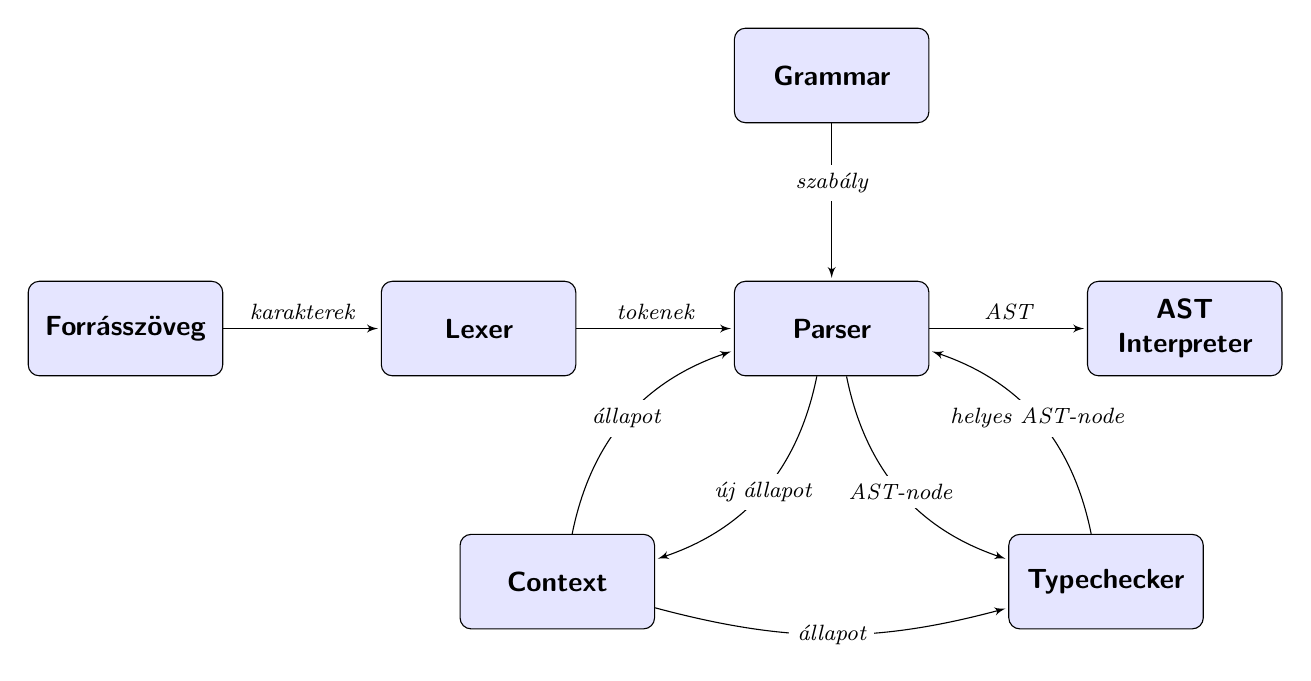
\begin{tikzpicture}[node distance=1cm,
	every node/.style={node distance=2cm, },
	clas/.style={rectangle, rounded corners, draw, fill=blue!10, inner sep=1pt, text width=2.4cm, text badly centered, minimum height=1.2cm, font=\bfseries\sffamily},
	arr/.style={->, >=latex', shorten >=1pt}
	]

\node[clas] (parser) {Parser};
\node[clas, above=of parser] (grammar) {Grammar};
\node[clas, left=of parser] (lexer) {Lexer};
\node[clas, below left=2 and 1 of parser] (context) {Context};
\node[clas, below right=2 and 1 of parser] (typechecker) {Typechecker};

\node[clas, left=of lexer] (source) {Forrásszöveg};
\node[clas, right=of parser] (interpreter) {AST Interpreter};

\path[arr, every node/.style={font=\itshape\footnotesize,
  		fill=white,inner sep=3pt}]
(source) edge node[above] {karakterek} (lexer)
(parser) edge [bend left=30] node {új állapot} (context)
(context) edge[bend left=30] node {állapot} (parser)
(grammar) edge node[above] {szabály} (parser)
(lexer) edge  node[above] {tokenek} (parser)
(parser) edge[bend right=30] node {AST-node} (typechecker)
(typechecker) edge[bend right=30] node {helyes AST-node} (parser)
(context) edge[bend right=15] node {állapot} (typechecker)
(parser) edge node[above] {AST} (interpreter);

\end{tikzpicture}
}
	\caption{A prototípus idealizált adatfolyam diagramja.}
\end{figure}


\subsubsection{A nyelvtan megadása}
A fordítóprogram által használt nyelvtant egy \cls{Grammar} objektumban adjuk meg: viszonylag szép, deklaratív szintaxissal sorolhatjuk meg a nyelv által használt lexikális elemeket a hozzájuk tartozó felszíni formákkal (ezek karaktersorozatok vagy reguláris kifejezések), beépített függvényeket, operátorokat.
A nyelvtan helyettesítési szabályait egy rekurzív leszállásos elemző függvényeiként adjuk meg.

\subsubsection{Lexikális elemzés}
A \cls{Lexer} a forrásszöveget bontja fel szimbólumokra a \cls{Context}ben tárolt szimbólumlista alapján.
Implementációja nagyon egyszerű: a forrásszöveg bemeneti karakterfolyamára megpróbáljuk ráilleszteni a szimbólumokat leíró reguláris kifejezéseket, majd a leghosszabb egyezést tekintjük találatnak, és ezt adjuk fel a \cls{Parser}nek.
Ezt az implementációt eleinte ideiglenesnek szántam, de a feladathoz mérten hatékonynak és megbízhatónak bizonyult.

Fontos megjegyezni, hogy a \cls{Lexer} valójában nem szimbólumokat ad vissza, hanem \cls{Token}eket.
A \cls{Token} rekord tartalmazza a szimbólumot, a tulajdonképpeni karaktersorozatot, illetve a karaktersorozat előfordulásának helyét a szövegben.

\subsubsection{Szintaktikus elemzés}
A \cls{Parser} a szintaktikus elemzést a \cls{Grammar} \cls{S} metódusának hívásával kezdi meg, ahonnan a nyelvtan szabályfüggvényeinek rekurzív hívásaival megy tovább.
Ezen szabályfüggvények visszatérési értéke egy \cls{Node}, azaz az absztrakt szintaxisfa egy csomópontja.

A megvalósított absztrakt szintaxisfa reguláris és heterogén: ,,heterogén'' mert a csomópontok különféle típusúak (külön leszármazott osztály valósítja meg például a feltételes utasítást és a kifejezést), és ,,reguláris'' mert a csomópontokat egységes, homogén interface-en keresztül is lehet kezelni.

\subsubsection{Szimbólumtábla}
A szimbólumtáblát a \cls{Context} osztály valósítja meg. Minden nevesített szemantikai egységet (típusokat, változókat, függvényeket) egy közös LeBlanc-Cook szimbólumtáblában tárol\cite[lásd][30]{ScottProgPrag}, de heterogén interface-t biztosít.

\subsubsection{Szemantikus elemzés}
A \cls{Grammar} egy szabályfüggvénye kérheti egy \cls{Node} szemantikus ellenőrzését a rosszul elnevezett \cls{ASTTypechecker} osztálytól.
Az \cls{ASTTypechecker} ellenőrzi az adott \cls{Node} és leszármazottai típushelyességét, és megkísérli rezolválni a függvényhívásokat.
A prototípus kezeli a túlterhelt függvényeket: a PLanG operátorai mind túlterhelt függvényként vannak megvalósítva.

\subsubsection{Interpreter}
Az elkészült, típushelyes absztrakt szintaxisfát az \cls{ASTInterpreter} osztály segítségével tudjuk futtatni.
Az \cls{ASTInterpreter} közvetlenül a szintaxisfát bejárva hajtja végre a programot.



\subsection{A tervezési döntések utólagos értékelése} \label{subsec:planres}
Ebben a részben \aref{subsec:plans} részben ismertetett tervezési döntéseket fogom értékelni.

Szép cél volt ugyan az, hogy minden PLanG program legyen érvényes XPLanG program is, de emiatt az XPLanGban is megjelennek a PLanG legnagyobb felhasználhatósági problémái, az alacsony szerepkifejező erejű kulcsszavak és a deklarációs lista.
A változtatható lexikális elemek a kulcsszavak problémájára megoldást nyújtanak, de a deklarációs lista súlyos problémái megmaradtak.

Nem volt egészen szerencsés választás a Java sem: a korlátlan hordozhatóság szép cél ugyan, de hasonló eredményt érünk el, ha a népszerű operációs rendszerekre fordított bináris állományokat terjesztjük, az egzotikusabb rendszerekhez pedig biztosítjuk a fordítás lehetőségét.

Ezzel szemben gondot okozott, hogy a Java virtuális gép indulása sok időt vesz igénybe, így a Javában írt parancssoros fordítóprogram növeli a nyelv effektív viszkozitását.
A Java határozott objektumorientáltsága is gyakran nehezítette a tisztán imperatív XPLanG fejlesztését, többször objektumelvű gondolatok szivárogtak bele a tervezésbe; ez különösen a típusrendszer alakításánál jelentett gondot.
De ha már Javát használtam, sok gondot megspórolhattam volna külső könyvtárak szabadabb használatával: függőségkezelő eszközök használatával a külső könyvtárak kezelése kezdőknek sem nehéz feladat.
Szintén érdemes lett volna kihasználni a Java 8 nyújtotta lehetőségeket.

Nem volt rossz döntés viszont saját elemzőt készíteni: nem került sokkal időbe, mint egy parsergenerátor használatát tisztességesen elsajátítani, és valóban nagyobb kontrollom volt így a hibaüzenetek generálásában, az elemzés logikai folyamatát is egyszerűsíteni tudtam, és rengeteget tanultam.

Az, hogy egyszerű fordítóprogram helyett egyfajta keretrendszert írtam komolyan megnehezítette és lassította a fejlesztést.
Egyértelműen a túlzott generalizáció csapdájába estem, minden tekintetben célszerűbb lett volna egy csak az XPLanGot értelmező fordítóprogramot írni.



\newpage
\printbibliography[heading=bibintoc]

\end{document}